\subsection{Użytkownicy udostępniający}
Następnym krokiem analizy kont, było dokonanie badania użytkowników udostępniających posty. Jak powiedziano wcześniej, analiza nie będzie dotyczyła szczegółów użytkowników ze względu na ich prywatność. Skupiono się jedynie na ich zachowaniu względem analizowanych kont. Łącznie dla 15? Tysięcy postów pobrano 11 tysięcy unikalnych użytkowników. Stworzono analizę, badającą średnie zachowanie tych użytkowników. Należy jednak zaznaczyć, że są to grupy użytkowników udostępniający posty danej klasy, ale nie oznacza to, że wyłącznie tej jednej klasy. 
\par
Najbardziej aktywnymi użytkownikami są Ci udostępniający posty kont oznaczonych jako nierzetelne. Średnio użytkownik z\,tej grupy udostępnił 10 postów ze zbioru zebranych nierzetelnych postów. Dla porównania średnia liczba udostępnień przez użytkownika postów typu mainstream to niecałe 5 postów.  Użytkownik, który dokonał maksymalnej liczby udostępnień wśród zebranych postów udostępnił 1900 tweetów z\,klasy nierzetelne. 
\par
Dla wszystkich klas łącznie średnia liczba udostępnień przez użytkownika wynosi 6 ale mediana wynosi już tylko 2 posty na użytkownika. Dodatkowo ciekawym jest, że ponad 45\% wszystkich użytkowników udostępniło tylko jeden post.  

\begin{table}[!h]
\centering 
\caption{Porównanie liczby oryginalnych tweetów do wszystkich tweetów danej klasy.} \label{tab:liczbaretweeterow}
\begin{tabular}{|m{2,8cm}|R{2,5cm}|R{2,5cm}|R{2,5cm}|R{2,5cm}|} 
\hline
Klasa kont & tweety & Unikalni użytkownicy & Max udostępnienia /użytkownika & Średnio udostępnienia/użytkownika \\ 
\hline
JUNK & 5685 & 4217 & 1962 & 9.9 \\ 
\hline
MAINSTREAM \textless{} 0,5mln & 5539 & 5311 & 842 & 4.0 \\ 
\hline
MAINSTREAM \textgreater{} 0,5mln & 4425 & 6718 & 1019 & 5.2 \\ 
\hline
FACTCHECK & 384 & 1994 & 67 & 2.9 \\
\hline
\end{tabular}
\end{table}

\subsubsection{Aktywność użytkowników udostępniających}
Dla wszystkich klas łącznie średnia liczba udostępnień przez użytkownika wynosi 6\,ale mediana wynosi już tylko 2 posty na użytkownika. Na rysynku \ref{fig:retweets-per-user} przedstawiono wykresy kołowe ukazujące jaki procent użytkowników udostępnił określoną liczbę postów z\,danej klasy. Dzięki rysunkowi wyraźnie widać, że ponad połowa użytkowników udostępniła maksymalnie dwa posty ze zbioru z\,każdej klasy. Tylko niewielki procent użytkowników udostępniał nie mniej niż 10 postów z\,danej klasy. Jednak największy procent takich użytkowników należy do klasy postów nierzetelnych. Dodatkowo jest, że ponad 45\% wszystkich użytkowników udostępniło tylko jeden post gdy brano pod uwagę wszystkie posty niezależnie od klasy do której należą.
\begin{figure}[!h]
	\centering 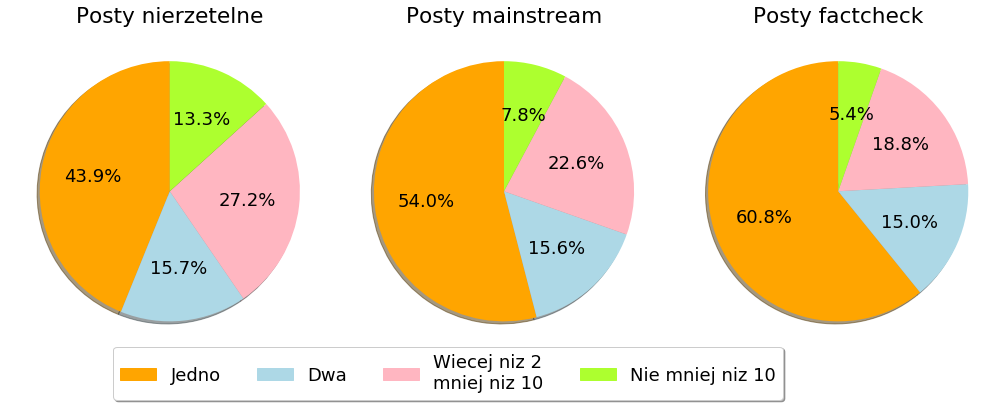
\includegraphics[width=0.95\linewidth]{img/results/retweetsperuser.png}
	\caption{Procent użytkowników z\,określoną liczbą udostępnień postów z\,danej klasy.} \label{fig:retweets-per-user}
\end{figure}

